\documentclass[a4paper,12pt]{article}
% Package to make citations superscrit with brackets
\usepackage[super,square]{natbib}
% Package to change margin size
\usepackage{anysize}
\marginsize{2cm}{2cm}{1cm}{2cm}
% Package to make headers
\usepackage{fancyhdr}
\renewcommand{\headrulewidth}{0pt}
% Package for highligths
\usepackage{soul}
% Colors for the references links
\usepackage[dvipsnames]{xcolor}
\usepackage{graphicx}
% Package to link references
\usepackage{hyperref}
\hypersetup{
    colorlinks=true,
    linkcolor=black,
    citecolor=CadetBlue,
    filecolor=CadetBlue,      
    urlcolor=CadetBlue,
}
% Package for lorem ipsum
\usepackage{lipsum}
% Package for multicolumn
\usepackage{multicol}

% Required package
\usepackage{amsmath, bm}
\setlength\columnsep{18pt}
% Sets bastract
\renewenvironment{abstract}
 {\par\noindent\textbf{\abstractname}\ \ignorespaces \\}
 {\par\noindent\medskip}



 
\begin{document}
% Makes header
\pagestyle{fancy}
\thispagestyle{empty}
\fancyhead[R]{\textit{Baltic Security Foundation}}
\fancyhead[L]{}
% Makes footnotes with an asterisk
\renewcommand*{\thefootnote}{\fnsymbol{footnote}}
\begin{center}
\Large{\textbf{Static Conformation of Star Polymer in Solvents of Varying Quality}}
\vspace{0.4cm}
\normalsize
\\ Ph.D. student: Reyhaneh Farimani, \ Supervisor: Christos Likos \\
\vspace{0.1cm}
\textit{University of Vienna}
\medskip
\normalsize
\end{center}
{\color{gray}\hrule}
\vspace{0.4cm}
\begin{abstract}
As part of my Ph.D. work in August 2023, I have prepared a report on the behavior of star polymers in solvents with varying quality. This section is taken from another part of my work and is now available in a public mode on a GitHub repository at \href{https://github.com/ReyhanehFarimani/LJLJ_potential.git}{This Git-Hub Repository}.

The report aims to replicate the findings of Huissmann \textit{et al.}~\cite{Huissmann2009} and analyze the behavior of star polymers under different solvent conditions. Its primary purpose is to verify the accuracy of the new pair potential designed for the Lammps MD package~\cite{LAMMPS}.
\end{abstract}
{\color{gray}\hrule}
\medskip
\section{Introduction}
Multiple studies have used a modified version of Lennard-Jones potential to find the Boyle point of the colloids, at which the second virial coefficient between two such particular molecules becomes zero. And the dependence of their behavior on the solvent quality~\cite{Huissmann2009, Zahra, Narros2013}.
\\
Until now, no one has ever added the pair potential usually used in these studies in the Lammps package. Herein, we have presented the potential, so if interested, you can add it in the following path: $\textit{/src/EXTRA-PAIR}$.
Compile the Lammps package again; note that you should also add the extra-pair package.

% % Theta point:
% The $\theta$ point for a gioiven system is defined as the \textit{Boyle point}. 
% The point at which the seocnd virial coefficient between two such particular molecules become zero.
% For a fixed Hamiltonian it will be depend on N and f at the same time.
% The Boyle point becomes independent of the topology in the limit of $N \to \infty$.
% % Worsen the solvent quality
% When the solvent's quality worsens, the monomers' effective attraction increases.
% The associated changes in the form of and effective interactions between thermal stars are of high interest because of the possibilities that open up in steering macroscopic properties via temperature change.
% % Star polymers:
% Bishop and Clarke, employed Brownian Dynamics to examine the scaling laws for radius gyration they found,
% $R^2_g \propto N^{6/5}$ for athermal solvent,
% $R^2_g \propto N$ for $Theta$ solvent,
% $R^2_g \propto N^{2/3}$ for fully collapsed state.
% In fully agreement with Flory expenses.
% % effective interaction:
% The star-star interaction is most certainly affected by the solvent quality.
% Field-theoretical model -> Benhamou \textit{et al.}
% Effective interaction around the $\Theta$ point -> Good description of SANS data. (Likos \textit{et al.})
% The importance:
% Adsorption of the star into surfaces, reversible gelation, and dynamics of the solutions.


\input{./sections/2_section.tex}
\section{Results}
\subsection{Comparing with extreme case}
As it is obvious the two cases of $\lambda = 0$, and $\lambda = 1$, are actually regular (shifted) Lennard-Jones Potential. The $\lambda = 0$ case, is the Lennard-Jones potential, truncated at $2^{1/6} \sigma$, and the 
$\lambda = 1$, is the usual Lennard-Jones potential.
\\
The best way to test if the potential is functioning properly is to confirm that systems with the same initial state and seed for the random number generator in the thermostat will follow the same path.
\\
We did the test for both cases and monitored the 
\begin{itemize}
    \item Temperature,
    \item Polymer Gyration Radius,
    \item Total Energy,
    \item System Trajectory.
\end{itemize}
In both cases, we have seen no difference between the pair potential manually added by us (\textit{LJ/LJ}), and the Lammps package \textit{LJ/CUT} pair potential.
\subsection{Finding $\Theta$ temperature}
After checking the result for the extreme cases, we are going to compare our result with the results in reference \cite{Huissmann2009}. In which we have compared the behavior of the radius of gyration with $\lambda$. The results are presented in figure \ref{fig:test}, \ref{fig:tes:normal}. Our results show the same behavior that was presented in the reference ~\cite{Huissmann2009}.
\begin{figure}
    \centering
    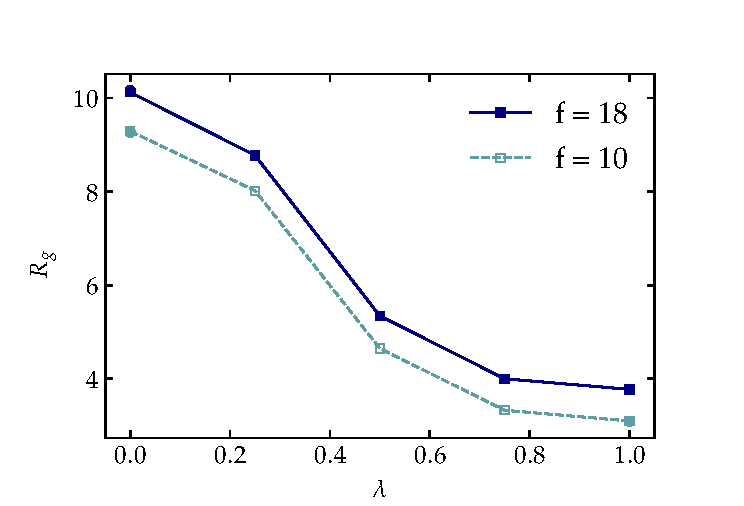
\includegraphics{figures/test_1.eps}
    \caption{Caption}
    \label{fig:test}
\end{figure}
\begin{figure}
    \centering
    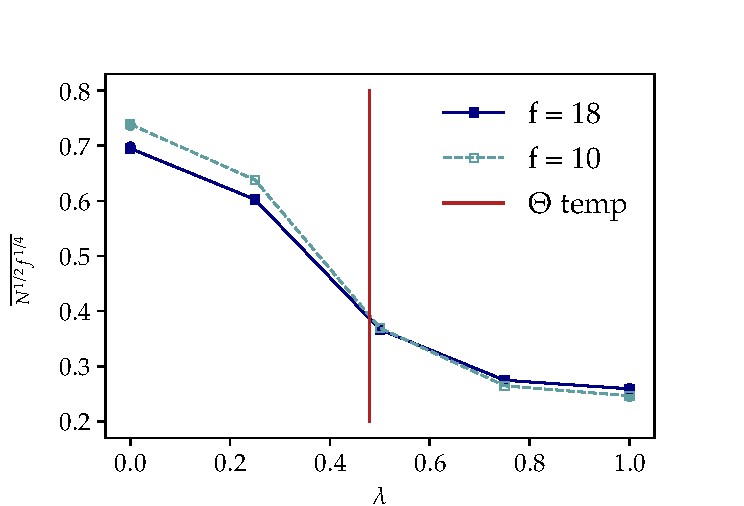
\includegraphics{figures/test_1_normalized.eps}
    \caption{Caption}
    \label{fig:tes:normal}
\end{figure}



\input{./sections/4_section.tex}
\section{Conclusion}
We obtained the correct behavior of star polymers in solvent with various qualities. The pair-potential added to the Lammps is correct, and this potential can be added to the Lammps extra-potential package, for future studies.
\bibliographystyle{plain}
\bibliography{references}
\end{document}